\documentclass[border=5pt]{standalone}
% Shared by every figure. Colour marks the TYPE of a quantity, never decoration:
%   blue   (vec) equivariant: rotates with its fragment     -- solid arrows
%   orange (inv) invariant: unchanged by any rotation        -- dashed arrows
%   aqua   (att) attention / communication between elements
%   violet (out) what the network outputs
% Text is always ink; a coloured mark next to it carries the meaning.
\usepackage{amsmath,amssymb,bm}
\usepackage{tikz}
\usetikzlibrary{arrows.meta,positioning,fit,backgrounds,calc,shapes.geometric,
  shapes.misc,decorations.pathreplacing,decorations.pathmorphing,matrix,
  patterns,cd,shadows}
\definecolor{vec}{HTML}{2A78D6}
\definecolor{inv}{HTML}{EB6834}
\definecolor{att}{HTML}{1BAF7A}
\definecolor{out}{HTML}{4A3AA7}
\definecolor{ink}{HTML}{0B0B0B}
\definecolor{ink2}{HTML}{52514E}
\definecolor{ink3}{HTML}{8A877F}
\definecolor{neutral}{HTML}{F0EFEC}
\definecolor{rule}{HTML}{CFCCC4}
\definecolor{pieceA}{HTML}{E4E1DA}
\definecolor{pieceB}{HTML}{CDC9BF}
\definecolor{pieceC}{HTML}{B3AEA2}
\colorlet{vecfill}{vec!9}
\colorlet{invfill}{inv!10}
\colorlet{attfill}{att!11}
\colorlet{outfill}{out!9}
\tikzset{
  >={Stealth[length=2.3mm,width=1.7mm]},
  every picture/.style={line cap=round, line join=round},
  box/.style={draw=ink2, fill=neutral, rounded corners=2.5pt, align=center,
    font=\small, inner sep=4pt, minimum height=8mm, text=ink, line width=0.6pt, nohyph},
  vecbox/.style={box, draw=vec, fill=vecfill},
  invbox/.style={box, draw=inv, fill=invfill},
  attbox/.style={box, draw=att, fill=attfill},
  outbox/.style={box, draw=out, fill=outfill},
  plain/.style={box, draw=ink3, fill=white},
  arr/.style={->, draw=ink2, line width=0.7pt},
  vecarr/.style={->, draw=vec, line width=1.1pt},
  invarr/.style={->, draw=inv, line width=1.1pt, dash pattern=on 3.2pt off 1.8pt},
  attarr/.style={->, draw=att, line width=1.1pt, dash pattern=on 1.2pt off 1.4pt},
  outarr/.style={->, draw=out, line width=1.1pt},
  nohyph/.style={execute at begin node={\hyphenpenalty=10000\exhyphenpenalty=10000\relax}},
  lbl/.style={font=\footnotesize, text=ink2, align=center, nohyph},
  tlbl/.style={font=\footnotesize, text=ink, align=center, nohyph},
  group/.style={draw=ink3, dashed, rounded corners=5pt, inner sep=7pt},
  op/.style={circle, draw=ink2, fill=white, inner sep=0pt, minimum size=5.2mm,
    font=\small, line width=0.6pt},
  piece/.style={fill=#1, draw=none},
  intact/.style={draw=ink2, line width=0.6pt},
  fracture/.style={draw=ink, line width=1.5pt},
  token/.style={circle, fill=att, draw=white, line width=0.5pt, inner sep=0pt,
    minimum size=4.2pt},
  vtx/.style={circle, fill=ink, inner sep=0pt, minimum size=3pt},
  panel/.style={font=\small\bfseries, text=ink, anchor=north west},
}
% one piece of the cartoon, in its own centred frame: fill, intact edge, fracture edge
\newcommand{\drawpiece}[2]{% #1 = A|B|C, #2 = fill colour
  \fill[#2] \csname Piece#1\endcsname;
  \draw[intact] \csname Intact#1\endcsname;
  \draw[fracture] \csname Crack#1\endcsname;}
% a legend entry: a short line in a given style, then its text
\newcommand{\legendline}[3]{% #1 position, #2 style, #3 text
  \draw[#2] (#1) -- ++(0.7,0) node[right, tlbl, text=ink] {#3};}

\def\FanDraw{\filldraw[fill=ink!9, draw=ink2, line width=0.5pt] (0.000,0.146) -- (-0.717,-0.288) -- (0.473,-0.808) -- cycle; \filldraw[fill=ink!8, draw=ink2, line width=0.5pt] (0.000,0.146) -- (0.473,-0.808) -- (0.898,-0.167) -- cycle; \filldraw[fill=ink!11, draw=ink2, line width=0.5pt] (0.000,0.146) -- (-1.116,0.145) -- (-0.717,-0.288) -- cycle; \filldraw[fill=ink!12, draw=ink2, line width=0.5pt] (0.000,0.146) -- (0.898,-0.167) -- (0.642,0.542) -- cycle; \filldraw[fill=ink!17, draw=ink2, line width=0.5pt] (0.000,0.146) -- (-0.181,0.334) -- (-1.116,0.145) -- cycle; \filldraw[fill=ink!17, draw=ink2, line width=0.5pt] (0.000,0.146) -- (0.642,0.542) -- (-0.181,0.334) -- cycle;}
\def\FanCoords{\coordinate (fv) at (0.000,0.146); \coordinate (fn) at (0.020,1.011); \coordinate (fo) at (-1.213,-1.502); \coordinate (fr0) at (0.898,-0.167); \coordinate (fr1) at (0.642,0.542); \coordinate (fr2) at (-0.181,0.334); \coordinate (fr3) at (-1.116,0.145); \coordinate (fr4) at (-0.717,-0.288); \coordinate (fr5) at (0.473,-0.808);}
\def\RoofDraw{\filldraw[fill=ink!10, draw=ink2, line width=0.5pt] (0.000,0.866) -- (0.000,-0.866) -- (1.141,-0.485) -- cycle; \filldraw[fill=ink!15, draw=ink2, line width=0.5pt] (0.000,-0.866) -- (0.000,0.866) -- (-1.301,-0.078) -- cycle;}
\def\RoofCoords{\coordinate (ru) at (0.000,-0.866); \coordinate (rv) at (0.000,0.866); \coordinate (r1) at (-0.434,-0.026); \coordinate (r2) at (0.380,-0.162); \coordinate (r1n) at (-0.738,0.450); \coordinate (r2n) at (0.859,0.277); \coordinate (ruo) at (0.189,-0.826); \coordinate (rvo) at (0.189,0.906);}
\def\RoofOrder{ab}
\def\RoofCos{0.69}

\begin{document}
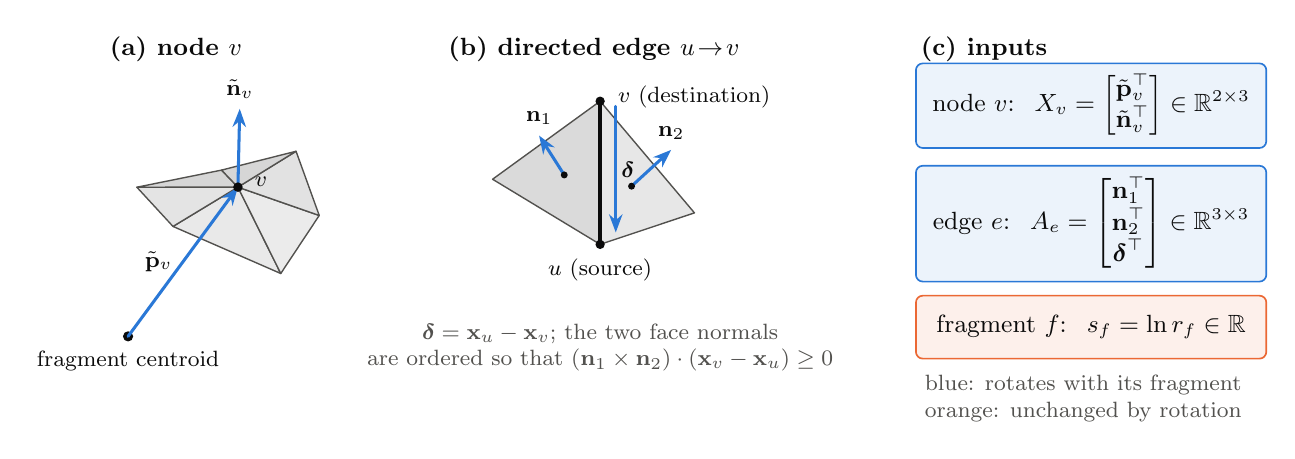
\begin{tikzpicture}
  % ---------------- (a) node features ----------------
  \begin{scope}[scale=1.15]
    \FanCoords
    \FanDraw
    \fill[ink] (fo) circle (1.6pt);
    \node[tlbl, anchor=north] at ($(fo)+(0,-0.05)$) {fragment centroid};
    \draw[vecarr] (fo) -- (fv) node[pos=0.5, left, tlbl] {$\tilde{\mathbf p}_v$};
    \draw[vecarr] (fv) -- (fn) node[above, tlbl] {$\tilde{\mathbf n}_v$};
    \fill[ink] (fv) circle (1.5pt);
    \node[tlbl, anchor=west] at ($(fv)+(0.08,0.06)$) {$v$};
  \end{scope}
  \node[panel] at (-1.75,2.2) {(a) node $v$};

  % ---------------- (b) edge features ----------------
  \begin{scope}[shift={(4.6,0.35)}, scale=1.05]
    \RoofCoords
    \RoofDraw
    \draw[ink, line width=1.2pt] (ru) -- (rv);
    \draw[vecarr] (r1) -- (r1n) node[above, tlbl] {$\mathbf n_1$};
    \draw[vecarr] (r2) -- (r2n) node[above, tlbl] {$\mathbf n_2$};
    \fill[ink] (r1) circle (1.2pt) (r2) circle (1.2pt);
    \draw[vecarr] ($(rvo)!0.06!(ruo)$) -- ($(rvo)!0.94!(ruo)$)
      node[pos=0.5, right, tlbl, inner sep=1.5pt] {$\boldsymbol\delta$};
    \fill[ink] (ru) circle (1.6pt) (rv) circle (1.6pt);
    \node[tlbl, anchor=north] at ($(ru)+(0,-0.06)$) {$u$ (source)};
    \node[tlbl, anchor=west] at ($(rv)+(0.1,0.05)$) {$v$ (destination)};
  \end{scope}
  \node[panel] at (2.55,2.2) {(b) directed edge $u\!\to\!v$};
  \node[lbl, anchor=north] at (4.6,-1.45)
    {$\boldsymbol\delta=\mathbf x_u-\mathbf x_v$; the two face normals\\ are ordered so that $(\mathbf n_1\times\mathbf n_2)\cdot(\mathbf x_v-\mathbf x_u)\ge 0$};

  % ---------------- (c) what the network receives ----------------
  \begin{scope}[shift={(8.6,1.75)}]
    \node[panel] at (-0.05,0.45) {(c) inputs};
    \node[vecbox, anchor=north west, align=left, minimum width=4.45cm] (x) at (0,0)
      {node $v$: \ $X_v=\begin{bmatrix}\tilde{\mathbf p}_v^{\top}\\ \tilde{\mathbf n}_v^{\top}\end{bmatrix}\in\mathbb R^{2\times 3}$};
    \node[vecbox, anchor=north west, align=left, minimum width=4.45cm] (a) at (0,-1.3)
      {edge $e$: \ $A_e=\begin{bmatrix}\mathbf n_1^{\top}\\ \mathbf n_2^{\top}\\ \boldsymbol\delta^{\top}\end{bmatrix}\in\mathbb R^{3\times 3}$};
    \node[invbox, anchor=north west, align=left, minimum width=4.45cm] (s) at (0,-2.95)
      {fragment $f$: \ $s_f=\ln r_f\in\mathbb R$};
    \node[lbl, anchor=north west, align=left] at (0,-3.85)
      {blue: rotates with its fragment\\ orange: unchanged by rotation};
  \end{scope}
\end{tikzpicture}
\end{document}
